\documentclass[tikz,border=2pt]{standalone}
\usepackage{amsmath}
\usepackage{pgfplots}
\pgfplotsset{compat=1.18}
\usetikzlibrary{arrows.meta}
\begin{document}
% Force of mortality within age 60 when p_60 = 0.9: CFM is flat at mu*_60 = -log 0.9 = 0.105;
% UDD has mu_{60+s} = 0.1/(1-0.1s), rising from 0.100 to 0.111. Both integrate to -log 0.9 over [0,1].
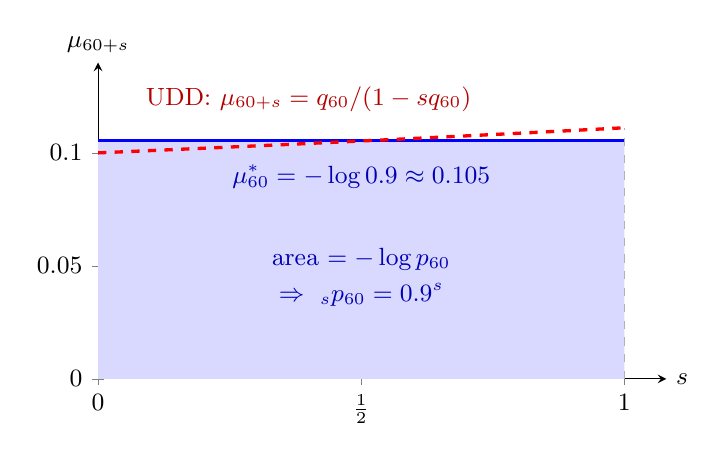
\begin{tikzpicture}[font=\small, >={Latex[length=2mm]}]
  \begin{axis}[
    axis lines=left, xmin=0, xmax=1.08, ymin=0, ymax=0.14,
    xtick={0,0.5,1}, xticklabels={$0$,$\tfrac12$,$1$},
    ytick={0,0.05,0.1}, yticklabels={$0$,$0.05$,$0.1$},
    xlabel={$s$}, ylabel={$\mu_{60+s}$},
    xlabel style={at={(axis description cs:1,0)}, anchor=west},
    ylabel style={rotate=-90, at={(axis description cs:0,1)}, anchor=south},
    samples=60, width=8.8cm, height=5.6cm, clip=false]
    \addplot[fill=blue!15, draw=none, domain=0:1] {0.10536} \closedcycle;
    \addplot[blue, very thick, domain=0:1] {0.10536};
    \addplot[red, very thick, dashed, domain=0:1] {0.1/(1-0.1*x)};
    \draw[gray!60, thin, dashed] (axis cs:1,0) -- (axis cs:1,0.1111);
    \node[blue!70!black, anchor=north] at (axis cs:0.5,0.099) {$\mu_{60}^*=-\log 0.9\approx0.105$};
    \node[red!70!black, anchor=south] at (axis cs:0.4,0.114) {UDD: $\mu_{60+s}=q_{60}/(1-sq_{60})$};
    \node[blue!70!black, align=center] at (axis cs:0.5,0.045) {area $=-\log p_{60}$\\[2pt]$\Rightarrow\ {}_sp_{60}=0.9^s$};
  \end{axis}
\end{tikzpicture}
\end{document}
